%        File: report.tex
%     Created: Tue Jun 09 02:00 PM 2015 C
% Last Change: Tue Jun 09 02:00 PM 2015 C
%
\documentclass[12pt]{scrreprt}
\usepackage[utf8]{inputenc}
\usepackage [backend=bibtex]{biblatex}
\addbibresource{bibliography.bib}
\usepackage{graphicx}
\graphicspath{ {images/} }
\usepackage[autostyle]{csquotes}
\usepackage{caption}
\usepackage{subcaption}
\usepackage{mathtools}
\usepackage{listings}
\begin{document}
To learn how cooperative behaviors may influence success ratio in a particular task, the decision was made to first observe the evolution in case where agents work against one another, competing for a higher score. Only then, comparing the results with those of a cooperative case, conclusions regarding cooperation influence may be drawn.

The scenarios were tested in parallel with each change, were it to complicate the problem or put emphasis on certain components of the solutions.

The two scenarios shall be described in their dedicated sections below, focusing on key contrast points. Following, however, are the elements common to both cases.

Evaluation process of candidate solutions was made in the same environment, with identical starting points and resource markers' locations. In both scenarios, trees produced by Genetic Programming are accompanied by a unchanging, user-defined tree in the simulations. This reference agent uses one type of Action, \textit{goToFlag(flagNumber)}, visiting each resource marker in turn, capturing them from first to last, never changing path between simulations. Figure \ref{fig:x referenceagentdiagram} presents the Behavior Tree schematic of the reference agent. Existence of such tree could fill the function of both a pressuring component (reflected in the fitness function in the appropriate cases) and essentialy a time-gate, as gathering all markers would end the simulation. Furthermore, algorithms in both cases had access to identical Behavior Tree Components to build the trees from, thus ensuring equal sophistication of solutions in each scenario.

\begin{figure}[h]
    \centering
    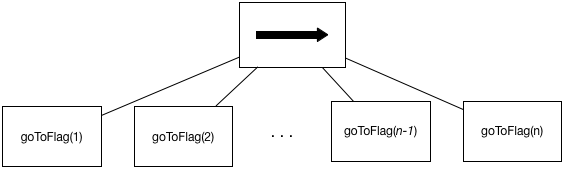
\includegraphics[scale=0.4]{referenceagentdiagram}
    \caption{A schematic of reference agent used in simulations.}
    \label{fig:x referenceagentdiagram}
\end{figure}
\section{Competitive Scenario Specification}
\subsection{Synopsis}
Competitive case assumed the optimal solution to the problem is maximizing the agent's personal gain. The markers gathered were counted for each agent separately, thus turning the task into a race - evolutionary agent was forced to get to as many markers as possible before the reference agent would claim them for himself.

After initial testing, the scenario was modified to feature 7 resource markers (instead of initial 5) and modified spawn points of agents -  readjusted to move evolutionary agent further back from the first marker. While increasing the number of markers served as an attempt to complicate the problem, moving evolutionary agent further from the first flag was done in the interest of being able to reproduce the results: since both agents were in the equal distance of the first flag and moved with the same speed, the matter of which one would claim the first flag was comparable to a coin-toss. Figure \ref{fig:x scenario1topdown} presents the final view of the competitive scenario map.

\begin{figure}[h]
\end{document}
